\documentclass[11pt]{article}
\usepackage[margin=1.0in]{geometry}
\usepackage{mathtools}
\usepackage{graphicx}
\usepackage{float}
\usepackage[font=small]{caption}
\usepackage{color}
\usepackage{fancyhdr}
%\usepackage{soul} %for striking out text
%\usepackage{arydshln} % for dotted line on truth table
\usepackage{tikz} % graphics stuff
\usepackage{caption}
\usepackage{gensymb}
\usepackage{booktabs}
\usepackage{listings}
\usepackage{fancyvrb}
%\usepackage{subcaption} % used to horizontally tile figures
%\usepackage{listings}
\pagestyle{fancy}
\fancyhead{}
\fancyfoot{}
\fancyfoot[R]{\thepage}

\definecolor{mygreen}{rgb}{0,0.6,0}
\definecolor{mygray}{rgb}{0.5,0.5,0.5}
\definecolor{mymauve}{rgb}{0.58,0,0.82}

\lstset{ 
	backgroundcolor=\color{white},   % choose the background color; you must add \usepackage{color} or \usepackage{xcolor}; should come as last argument
	basicstyle=\footnotesize,        % the size of the fonts that are used for the code
	breakatwhitespace=false,         % sets if automatic breaks should only happen at whitespace
	breaklines=true,                 % sets automatic line breaking
	captionpos=t,                    % sets the caption-position to bottom
	commentstyle=\color{mygreen},    % comment style
	deletekeywords={},               % if you want to delete keywords from the given language
	escapeinside={\%*}{*)},          % if you want to add LaTeX within your code
	extendedchars=false,             % lets you use non-ASCII characters; for 8-bits encodings only, does not work with UTF-8
	firstnumber=0,                   % start line enumeration with line 1000
	frame=single,                    % adds a frame around the code
	keepspaces=true,                 % keeps spaces in text, useful for keeping indentation of code (possibly needs columns=flexible)
	keywordstyle=\color{blue},       % keyword style
	language=VHDL,                   % the language of the code
	morekeywords={},                 % if you want to add more keywords to the set
	numbers=left,                    % where to put the line-numbers; possible values are (none, left, right)
	numbersep=5pt,                   % how far the line-numbers are from the code
	numberstyle=\tiny\color{mygray}, % the style that is used for the line-numbers
	rulecolor=\color{black},         % if not set, the frame-color may be changed on line-breaks within not-black text (e.g. comments (green here))
	showspaces=false,                % show spaces everywhere adding particular underscores; it overrides 'showstringspaces'
	showstringspaces=false,          % underline spaces within strings only
	showtabs=false,                  % show tabs within strings adding particular underscores
	stepnumber=5,                    % the step between two line-numbers. If it's 1, each line will be numbered
	stringstyle=\color{mymauve},     % string literal style
	tabsize=4, 	                     % sets default tabsize to 2 spaces
	title=\lstname                   % show the filename of files included with \lstinputlisting; also try caption instead of title
}

\begin{document}

%
% cover page
%

\vspace*{2 cm}

\begin{center}
\bf{CMPE-630 Digital IC Design\\
    Laboratory Exercise 7\\
\vspace{0.25 cm}
Autolayout Design Techniques (HDL-Layout)
}
\end{center}

\vspace{6 cm}

\begin{flushright}
Brandon Key and Chris Guarini\\
Performed: 9 Dec 2019\\
Submitted: 9 Dec 2019\\
\vspace{0.5 cm}
Instructor: Dr. Amlan Ganguly\\
TAs: Abhishek Vashist\\
Andrew Fountain\\
Piers Kwan\\
\vspace{0.5 cm}
\end{flushright}

\vspace{3 cm}
\indent By submitting this report, you attest that you neither have given nor have received any assistance (including writing, collecting data, plotting figures, tables or graphs, or using previous student reports as a reference), and you further acknowledge that giving or receiving such assistance will result in a failing grade for this course.

\vspace{1 cm}
Your Signature:   \rule{13cm}{.1pt}


\tableofcontents
\newpage

\section{Abstract}

	Integrated Circuit Design is a costly and complex endeavor. Fortunately, automatic tools speed up the process and allow designs that are not possible to create manually. This exercise implemented a 1-Bit ALU and a 16-Bit ALU using autolayout. The autolayout tools generated very reasonable circuits. The 1-Bit ALU has an input frequency of 380.92MHz and a throughput frequency of 553.4MHz, while the 16-bit ALU has an input frequency of 461.02MHz and a throughput frequency of 110.2MHz. The area used by the ALUs was also reasonable with the 1-bit ALU taking up 647.89$\mu m^2$ and the 16-bit ALU occupying 9792.5$\mu m^2$.
	

\section{Design Methodology and Theory}

	A cornerstone of IC design is the ability to create large, complex designs from smaller more manageable parts. The project outlined in this exercise calls for the design, testing and layout of a multiply and accumulate (MAC) unit, which takes two 16-bit inputs, multiplies them together, adds them to the value stored in a register, and then stores that output back into the register. The final component should contain a built in self test (BIST) that verifies the functionality of the MAC.
	
	The MAC is composed of a carry-save multiplier, ripple carry full-adder, and parallel register. The BIST is implemented through the use of an LFSR for the inputs, an MISR for the output, and a test controller which controls the timing and sets the test passed and test complete outputs. A full diagram of the MAC with BIST can be seen below in \textit{Figure 1}.
	
	\begin{figure}
		\centering
		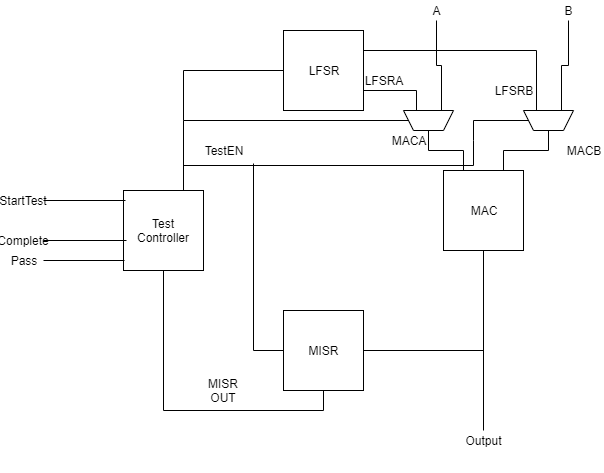
\includegraphics[width=0.7\linewidth]{Pictures/Full-Project-Block}
		\caption{\textbf{Figure 1: } High Level Block Diagram of the MAC with BIST.}
		\label{fig:full-project-block}
	\end{figure}
	

	

\section{Results and Analysis}
		
	\begin{figure}[H] 
		\centering 
		\includegraphics[width=0.7\linewidth]{"Pictures/Full Schematic Page 7"}
		\caption{Full Schematic Page 7} 
		\label{fig:Full-Schematic-Page-7} 
	\end{figure}
	
	
	\begin{figure}[H] 
		\centering 
		\includegraphics[width=0.7\linewidth]{"Pictures/Full-Project-Block"}
		\caption{Full Project Block} 
		\label{fig:Full-Project-Block} 
	\end{figure}
	
	
	\begin{figure}[H] 
		\centering 
		\includegraphics[width=0.7\linewidth]{"Pictures/Full Layout"}
		\caption{Full Layout} 
		\label{fig:Full-Layout} 
	\end{figure}
	
	
	\begin{figure}[H] 
		\centering 
		\includegraphics[width=0.7\linewidth]{"Pictures/Full Schematic Page 8"}
		\caption{Full Schematic Page 8} 
		\label{fig:Full-Schematic-Page-8} 
	\end{figure}
	
	
	\begin{figure}[H] 
		\centering 
		\includegraphics[width=0.7\linewidth]{"Pictures/Full Schematic Page 2"}
		\caption{Full Schematic Page 2} 
		\label{fig:Full-Schematic-Page-2} 
	\end{figure}
	
	
	\begin{figure}[H] 
		\centering 
		\includegraphics[width=0.7\linewidth]{"Pictures/Multiplier Schematic Page 2"}
		\caption{Multiplier Schematic Page 2} 
		\label{fig:Multiplier-Schematic-Page-2} 
	\end{figure}
	
	
	\begin{figure}[H] 
		\centering 
		\includegraphics[width=0.7\linewidth]{"Pictures/Full Layout Close Up View"}
		\caption{Full Layout Close Up View} 
		\label{fig:Full-Layout-Close-Up-View} 
	\end{figure}
	
	
	\begin{figure}[H] 
		\centering 
		\includegraphics[width=0.7\linewidth]{"Pictures/BIST-Test-Bench"}
		\caption{BIST Test Bench} 
		\label{fig:BIST-Test-Bench} 
	\end{figure}
	
	
	\begin{figure}[H] 
		\centering 
		\includegraphics[width=0.7\linewidth]{"Pictures/Full Schematic Page 17"}
		\caption{Full Schematic Page 17} 
		\label{fig:Full-Schematic-Page-17} 
	\end{figure}
	
	
	\begin{figure}[H] 
		\centering 
		\includegraphics[width=0.7\linewidth]{"Pictures/Full Schematic Page 6"}
		\caption{Full Schematic Page 6} 
		\label{fig:Full-Schematic-Page-6} 
	\end{figure}
	
	
	\begin{figure}[H] 
		\centering 
		\includegraphics[width=0.7\linewidth]{"Pictures/nBitAdder Schematic Page 1"}
		\caption{nBitAdder Schematic Page 1} 
		\label{fig:nBitAdder-Schematic-Page-1} 
	\end{figure}
	
	
	\begin{figure}[H] 
		\centering 
		\includegraphics[width=0.7\linewidth]{"Pictures/Full Schematic Page 27"}
		\caption{Full Schematic Page 27} 
		\label{fig:Full-Schematic-Page-27} 
	\end{figure}
	
	
	\begin{figure}[H] 
		\centering 
		\includegraphics[width=0.7\linewidth]{"Pictures/Full Schematic Page 15"}
		\caption{Full Schematic Page 15} 
		\label{fig:Full-Schematic-Page-15} 
	\end{figure}
	
	
	\begin{figure}[H] 
		\centering 
		\includegraphics[width=0.7\linewidth]{"Pictures/Full Schematic Page 19"}
		\caption{Full Schematic Page 19} 
		\label{fig:Full-Schematic-Page-19} 
	\end{figure}
	
	
	\begin{figure}[H] 
		\centering 
		\includegraphics[width=0.7\linewidth]{"Pictures/nBitRegister 16-Bit Schematic"}
		\caption{nBitRegister 16 Bit Schematic} 
		\label{fig:nBitRegister-16-Bit-Schematic} 
	\end{figure}
	
	
	\begin{figure}[H] 
		\centering 
		\includegraphics[width=0.7\linewidth]{"Pictures/Full Schematic Page 20"}
		\caption{Full Schematic Page 20} 
		\label{fig:Full-Schematic-Page-20} 
	\end{figure}
	
	
	\begin{figure}[H] 
		\centering 
		\includegraphics[width=0.7\linewidth]{"Pictures/Full Schematic Page 24"}
		\caption{Full Schematic Page 24} 
		\label{fig:Full-Schematic-Page-24} 
	\end{figure}
	
	
	\begin{figure}[H] 
		\centering 
		\includegraphics[width=0.7\linewidth]{"Pictures/MAC-block"}
		\caption{MAC block} 
		\label{fig:MAC-block} 
	\end{figure}
	
	
	\begin{figure}[H] 
		\centering 
		\includegraphics[width=0.7\linewidth]{"Pictures/Full Schematic Page 5"}
		\caption{Full Schematic Page 5} 
		\label{fig:Full-Schematic-Page-5} 
	\end{figure}
	
	
	\begin{figure}[H] 
		\centering 
		\includegraphics[width=0.7\linewidth]{"Pictures/Full Schematic Page 16"}
		\caption{Full Schematic Page 16} 
		\label{fig:Full-Schematic-Page-16} 
	\end{figure}
	
	
	\begin{figure}[H] 
		\centering 
		\includegraphics[width=0.7\linewidth]{"Pictures/nBitAdder Schematic Page 2"}
		\caption{nBitAdder Schematic Page 2} 
		\label{fig:nBitAdder-Schematic-Page-2} 
	\end{figure}
	
	
	\begin{figure}[H] 
		\centering 
		\includegraphics[width=0.7\linewidth]{"Pictures/Full Schematic Page 26"}
		\caption{Full Schematic Page 26} 
		\label{fig:Full-Schematic-Page-26} 
	\end{figure}
	
	
	\begin{figure}[H] 
		\centering 
		\includegraphics[width=0.7\linewidth]{"Pictures/nBitMux_2to1 Schematic"}
		\caption{nBitMux 2to1 Schematic} 
		\label{fig:nBitMux-2to1-Schematic} 
	\end{figure}
	
	
	\begin{figure}[H] 
		\centering 
		\includegraphics[width=0.7\linewidth]{"Pictures/Full Schematic Page 1"}
		\caption{Full Schematic Page 1} 
		\label{fig:Full-Schematic-Page-1} 
	\end{figure}
	
	
	\begin{figure}[H] 
		\centering 
		\includegraphics[width=0.7\linewidth]{"Pictures/nBitRegister 32-Bit Layout"}
		\caption{nBitRegister 32 Bit Layout} 
		\label{fig:nBitRegister-32-Bit-Layout} 
	\end{figure}
	
	
	\begin{figure}[H] 
		\centering 
		\includegraphics[width=0.7\linewidth]{"Pictures/Full Schematic Page 9"}
		\caption{Full Schematic Page 9} 
		\label{fig:Full-Schematic-Page-9} 
	\end{figure}
	
	
	\begin{figure}[H] 
		\centering 
		\includegraphics[width=0.7\linewidth]{"Pictures/nBitRegister 16-Bit Layout"}
		\caption{nBitRegister 16 Bit Layout} 
		\label{fig:nBitRegister-16-Bit-Layout} 
	\end{figure}
	
	
	\begin{figure}[H] 
		\centering 
		\includegraphics[width=0.7\linewidth]{"Pictures/Full Schematic Page 23"}
		\caption{Full Schematic Page 23} 
		\label{fig:Full-Schematic-Page-23} 
	\end{figure}
	
	
	\begin{figure}[H] 
		\centering 
		\includegraphics[width=0.7\linewidth]{"Pictures/Full Schematic Page 28"}
		\caption{Full Schematic Page 28} 
		\label{fig:Full-Schematic-Page-28} 
	\end{figure}
	
	
	\begin{figure}[H] 
		\centering 
		\includegraphics[width=0.7\linewidth]{"Pictures/Full Schematic Page 22"}
		\caption{Full Schematic Page 22} 
		\label{fig:Full-Schematic-Page-22} 
	\end{figure}
	
	
	\begin{figure}[H] 
		\centering 
		\includegraphics[width=0.7\linewidth]{"Pictures/Full Schematic Page 14"}
		\caption{Full Schematic Page 14} 
		\label{fig:Full-Schematic-Page-14} 
	\end{figure}
	
	
	\begin{figure}[H] 
		\centering 
		\includegraphics[width=0.7\linewidth]{"Pictures/Full Schematic Page 13"}
		\caption{Full Schematic Page 13} 
		\label{fig:Full-Schematic-Page-13} 
	\end{figure}
	
	
	\begin{figure}[H] 
		\centering 
		\includegraphics[width=0.7\linewidth]{"Pictures/MAC-16bit-Test-Bench"}
		\caption{MAC 16bit Test Bench} 
		\label{fig:MAC-16bit-Test-Bench} 
	\end{figure}
	
	
	\begin{figure}[H] 
		\centering 
		\includegraphics[width=0.7\linewidth]{"Pictures/nBitRegister 32-Bit Schematic"}
		\caption{nBitRegister 32 Bit Schematic} 
		\label{fig:nBitRegister-32-Bit-Schematic} 
	\end{figure}
	
	
	\begin{figure}[H] 
		\centering 
		\includegraphics[width=0.7\linewidth]{"Pictures/Full Schematic Page 18"}
		\caption{Full Schematic Page 18} 
		\label{fig:Full-Schematic-Page-18} 
	\end{figure}
	
	
	\begin{figure}[H] 
		\centering 
		\includegraphics[width=0.7\linewidth]{"Pictures/MAC-Test-Bench"}
		\caption{MAC Test Bench} 
		\label{fig:MAC-Test-Bench} 
	\end{figure}
	
	
	\begin{figure}[H] 
		\centering 
		\includegraphics[width=0.7\linewidth]{"Pictures/Full Schematic Page 12"}
		\caption{Full Schematic Page 12} 
		\label{fig:Full-Schematic-Page-12} 
	\end{figure}
	
	
	\begin{figure}[H] 
		\centering 
		\includegraphics[width=0.7\linewidth]{"Pictures/Full Schematic Page 11"}
		\caption{Full Schematic Page 11} 
		\label{fig:Full-Schematic-Page-11} 
	\end{figure}
	
	
	\begin{figure}[H] 
		\centering 
		\includegraphics[width=0.7\linewidth]{"Pictures/Multiplier Schematic Page 1"}
		\caption{Multiplier Schematic Page 1} 
		\label{fig:Multiplier-Schematic-Page-1} 
	\end{figure}
	
	
	\begin{figure}[H] 
		\centering 
		\includegraphics[width=0.7\linewidth]{"Pictures/Full Schematic Page 21"}
		\caption{Full Schematic Page 21} 
		\label{fig:Full-Schematic-Page-21} 
	\end{figure}
	
	
	\begin{figure}[H] 
		\centering 
		\includegraphics[width=0.7\linewidth]{"Pictures/Full Schematic Page 4"}
		\caption{Full Schematic Page 4} 
		\label{fig:Full-Schematic-Page-4} 
	\end{figure}
	
	
	\begin{figure}[H] 
		\centering 
		\includegraphics[width=0.7\linewidth]{"Pictures/Full Schematic Page 3"}
		\caption{Full Schematic Page 3} 
		\label{fig:Full-Schematic-Page-3} 
	\end{figure}
	
	
	\begin{figure}[H] 
		\centering 
		\includegraphics[width=0.7\linewidth]{"Pictures/Full Schematic Page 25"}
		\caption{Full Schematic Page 25} 
		\label{fig:Full-Schematic-Page-25} 
	\end{figure}
	
	
	\begin{figure}[H] 
		\centering 
		\includegraphics[width=0.7\linewidth]{"Pictures/Full Schematic Page 10"}
		\caption{Full Schematic Page 10} 
		\label{fig:Full-Schematic-Page-10} 
	\end{figure}
	
	
	\begin{figure}[H] 
		\centering 
		\includegraphics[width=0.7\linewidth]{"Pictures/nBitMux_2to1 Layout"}
		\caption{nBitMux 2to1 Layout} 
		\label{fig:nBitMux-2to1-Layout} 
	\end{figure}
	
	
		
	\subsection{Layout}
		
	
	
	\subsection{Timing}
	

	
	\subsection{Power}
	
	
	 STATIC_PWR  = -1.8787E-06   
	INST_PWR    =  1.6029E-02   
	
	

			

\section{Conclusion}




\section{Appendix}

	\subsection{VHDL}
	
		\lstinputlisting[caption={MAC tb VHDL }\label{lst:MAC-tb-vhd}]{"SourceCode/MAC_tb.vhd"}
		
		\lstinputlisting[caption={ProjectWrapper tb VHDL }\label{lst:ProjectWrapper-tb-vhd}]{"SourceCode/ProjectWrapper_tb.vhd"}
		
		\lstinputlisting[caption={FullAdder VHDL }\label{lst:FullAdder-vhd}]{"SourceCode/FullAdder.vhd"}
		
		\lstinputlisting[caption={FA 1bit VHDL }\label{lst:FA-1bit-vhd}]{"SourceCode/FA_1bit.vhd"}
		
		\lstinputlisting[caption={AND2 VHDL }\label{lst:AND2-vhd}]{"SourceCode/AND2.vhd"}
		
		\lstinputlisting[caption={nBitRegister VHDL }\label{lst:nBitRegister-vhd}]{"SourceCode/nBitRegister.vhd"}
		
		\lstinputlisting[caption={Shifter VHDL }\label{lst:Shifter-vhd}]{"SourceCode/Shifter.vhd"}
		
		\lstinputlisting[caption={TestController VHDL }\label{lst:TestController-vhd}]{"SourceCode/TestController.vhd"}
		
		\lstinputlisting[caption={Subtractor VHDL }\label{lst:Subtractor-vhd}]{"SourceCode/Subtractor.vhd"}
		
		\lstinputlisting[caption={Controller VHDL }\label{lst:Controller-vhd}]{"SourceCode/Controller.vhd"}
		
		\lstinputlisting[caption={ProjectWrapper VHDL }\label{lst:ProjectWrapper-vhd}]{"SourceCode/ProjectWrapper.vhd"}
		
		\lstinputlisting[caption={Counter VHDL }\label{lst:Counter-vhd}]{"SourceCode/Counter.vhd"}
		
		\lstinputlisting[caption={BIST tb VHDL }\label{lst:BIST-tb-vhd}]{"SourceCode/BIST_tb.vhd"}
		
		\lstinputlisting[caption={Multiplier VHDL }\label{lst:Multiplier-vhd}]{"SourceCode/Multiplier.vhd"}
		
		\lstinputlisting[caption={LFSR 32 4 VHDL }\label{lst:LFSR-32-4-vhd}]{"SourceCode/LFSR_32_4.vhd"}
		
		\lstinputlisting[caption={LFSR 8 4 VHDL }\label{lst:LFSR-8-4-vhd}]{"SourceCode/LFSR_8_4.vhd"}
		
		\lstinputlisting[caption={MAC VHDL }\label{lst:MAC-vhd}]{"SourceCode/MAC.vhd"}
		
		\lstinputlisting[caption={MISR 32 4 VHDL }\label{lst:MISR-32-4-vhd}]{"SourceCode/MISR_32_4.vhd"}
		
		\lstinputlisting[caption={nBitRegister tb VHDL }\label{lst:nBitRegister-tb-vhd}]{"SourceCode/nBitRegister_tb.vhd"}
		
		\lstinputlisting[caption={nBitAdder VHDL }\label{lst:nBitAdder-vhd}]{"SourceCode/nBitAdder.vhd"}
		
		\lstinputlisting[caption={nBitRegister 16 VHDL }\label{lst:nBitRegister-16-vhd}]{"SourceCode/nBitRegister_16.vhd"}
		
		\lstinputlisting[caption={MISR 8 4 VHDL }\label{lst:MISR-8-4-vhd}]{"SourceCode/MISR_8_4.vhd"}
		
		\lstinputlisting[caption={nBitMux 2to1 VHDL }\label{lst:nBitMux-2to1-vhd}]{"SourceCode/nBitMux_2to1.vhd"}
		
		\lstinputlisting[caption={ANDADD VHDL }\label{lst:ANDADD-vhd}]{"SourceCode/ANDADD.vhd"}
		
		\lstinputlisting[caption={Ripple Carry FA VHDL }\label{lst:Ripple-Carry-FA-vhd}]{"SourceCode/Ripple_Carry_FA.vhd"}
		
		\lstinputlisting[caption={nBitRegister 32 VHDL }\label{lst:nBitRegister-32-vhd}]{"SourceCode/nBitRegister_32.vhd"}
		
		\lstinputlisting[caption={ALU Wrapper VHDL }\label{lst:ALU-Wrapper-vhd}]{"SourceCode/ALU_Wrapper.vhd"}
		
		\lstinputlisting[caption={nBitAdderSubtractor 16Bit VHDL }\label{lst:nBitAdderSubtractor-16Bit-vhd}]{"SourceCode/nBitAdderSubtractor_16Bit.vhd"}
		
		\lstinputlisting[caption={ALU TESTBENCH VHDL }\label{lst:ALU-TESTBENCH-vhd}]{"SourceCode/ALU_TESTBENCH.vhd"}
		
		\lstinputlisting[caption={Logic Unit VHDL }\label{lst:Logic-Unit-vhd}]{"SourceCode/Logic_Unit.vhd"}
		

	\subsection{Leonardo Scripts}
		
		\lstinputlisting[caption={Multiplier Spectrum Script }\label{lst:Multiplier-script}]{"LeonardoScripts/Multiplier.script"}
		
		\lstinputlisting[caption={LFSR 32 4 Spectrum Script }\label{lst:LFSR-32-4-script}]{"LeonardoScripts/LFSR_32_4.script"}
		
		\lstinputlisting[caption={MISR 32 4 Spectrum Script }\label{lst:MISR-32-4-script}]{"LeonardoScripts/MISR_32_4.script"}
		
		\lstinputlisting[caption={ProjectWrapper Spectrum Script }\label{lst:ProjectWrapper-script}]{"LeonardoScripts/ProjectWrapper.script"}
		
		\lstinputlisting[caption={nBitAdder Spectrum Script }\label{lst:nBitAdder-script}]{"LeonardoScripts/nBitAdder.script"}
		
		\lstinputlisting[caption={nBitAdderSubtractor Spectrum Script }\label{lst:nBitAdderSubtractor-script}]{"LeonardoScripts/nBitAdderSubtractor.script"}
		
		\lstinputlisting[caption={MAC BIST Spectrum Script }\label{lst:MAC-BIST-script}]{"LeonardoScripts/MAC-BIST.script"}
		
		\lstinputlisting[caption={nBitRegister 16 Spectrum Script }\label{lst:nBitRegister-16-script}]{"LeonardoScripts/nBitRegister_16.script"}
		
		\lstinputlisting[caption={MAC Spectrum Script }\label{lst:MAC-script}]{"LeonardoScripts/MAC.script"}
		
		\lstinputlisting[caption={nBitMux 2to1 Spectrum Script }\label{lst:nBitMux-2to1-script}]{"LeonardoScripts/nBitMux_2to1.script"}
		
		\lstinputlisting[caption={nBitRegister 32 Spectrum Script }\label{lst:nBitRegister-32-script}]{"LeonardoScripts/nBitRegister_32.script"}
		
		\lstinputlisting[caption={MAC (copy) Spectrum Script }\label{lst:MAC-(copy)-script}]{"LeonardoScripts/MAC (copy).script"}
		
		
	\subsection{SPICE}
	
		\lstinputlisting[caption={layout test SPICE }\label{lst:layout-test-spice}]{"Spice/layout_test.cir"}
		
		\lstinputlisting[caption={power test SPICE }\label{lst:power-test-spice}]{"Spice/power_test.cir"}
		

		
\section{References}

	Key, Brandon A. \textit{CMPE 260 Laboratory Exercise 3 Arithmetic Logic Unit}. CMPE 260 Laboratory Exercise 3 Arithmetic Logic Unit.
	
	// TODO add BIST from DSD II

\end{document}
